% !TEX root = results_only.tex

This chapter describes the results of several experimental setups.
First, we ran a control case, using a uniform population and a uniform intensity.
The results for the control case are described in \cref{sec:results:unif_100_unif}.
We then made ran several sets of experiments while changing one parameter at a time.
\Cref{sec:results:unif_NCases_1h} compares the results obtained by varying the number of cases.
\Cref{sec:results:unifNpop_100_1h} compares the results obtained by varying the size of the population.


\section{Control case - uniform risk on a uniform population}
\label{sec:results:unif_100_unif}

\Cref{tbl:errors:unif_100_unif} lists the mean error rates obtained for a uniform intensity with factor of 100, over a uniform population of 10,000.
The columns represent the errors observed by using the three different methods for computing the smoothing bandwidth:
the Oracle, the Silverman rule of thumb, and least-squares cross validation.

Each row represents a different measure of error.
The first row, MISE, is the mean integrated squared error.
Relative MISE is the mean integrated relative squared error, where the relative squared error is computed in the following manner:
\[ RSE(x) = \left(\frac{\hat{f}(x)-f(x)}{f(x)}\right)^2 \]
The next row is the mean integrated absolute error (MIAE), which is followed by Relative MIAE which is computed analogously to Relative MISE.
This is followed by the Maximum error, which is the greatest absolute error over the study area.

The error measures mentioned above each compare the closeness of the estimated intensity function to the true funcition.
The following error measures, on the other hand, relate the closeness of the \textit{peak} of the estimate to the true peak.
The \textit{peak bias} is the average difference between the computed and true maxima, that is the empirical expectation of \(\max{\{\hat{f}(x)\}} - \max{\{f(x)\}}\).
The Relative peak bias is peak bias expressed relative to the true maximum.
The \textit{peak drift} is the Euclidean distance between the estimated peak and the true peak.
The Relative peak drift is the peak drift, expressed relative to the width of the study area.

The next four measures, \textit{centroid bias} and \textit{drift}, and the relative versions of them, are analogous to the peak error measures.
However, instead of comparing the true peak to the peak of the estimate, they compare it to the location and value of the estimate, calculated at the centroid of the top five percent of the estimated function.


\begin{table}[H]
\centering
% latex table generated in R 3.3.3 by xtable 1.8-2 package
% Sun Mar 11 18:27:52 2018
\begin{tabular}{lrrr}
  \hline
 & Oracle & Silverman & CV \\ 
  \hline
MISE & 0.000012 & 0.000013 & 0.000013 \\ 
  Relative MISE & 0.116112 & 0.125979 & 0.128308 \\ 
  Normalized MISE & 0.000000 & 0.000000 & 0.000000 \\ 
  MIAE & 0.002786 & 0.002898 & 0.002938 \\ 
  Relative MIAE & 0.278620 & 0.289846 & 0.293819 \\ 
  Normalized MIAE & 0.000000 & 0.000000 & 0.000000 \\ 
  Max Error & 0.008551 & 0.009000 & 0.008926 \\ 
  Normalized Max Error & 0.000001 & 0.000001 & 0.000001 \\ 
   \hline
\end{tabular}

\caption{Mean error rates for uniform population, uniform intensity of factor 100}
\label{tbl:errors:unif_100_unif}
\end{table}

\begin{figure}[htb]
    \centering
    \begin{subfigure}[t]{0.45\textwidth}
    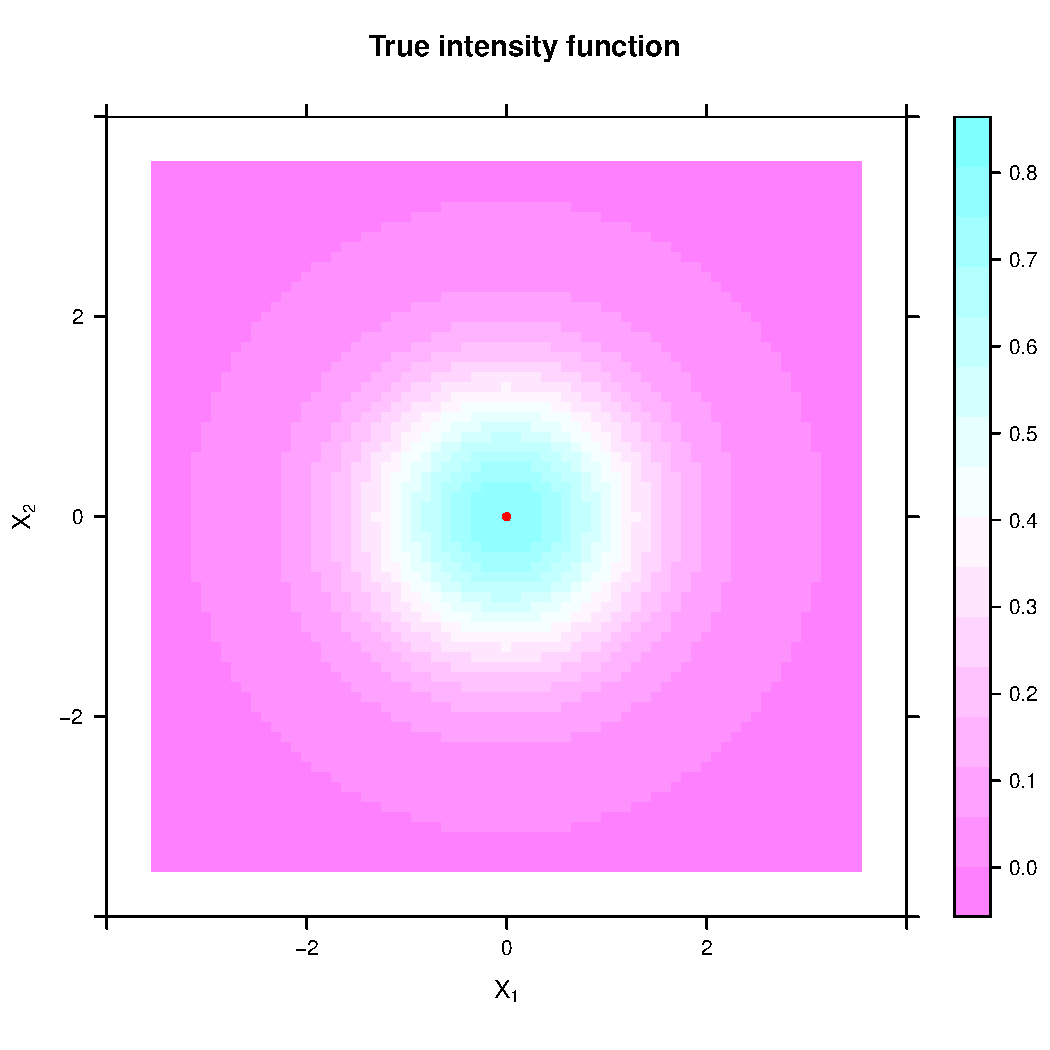
\includegraphics[width=\textwidth]{results/unif_100_unif/output/true_intensity_heatmap}
    \caption{True intensity}
    \end{subfigure}
    \begin{subfigure}[t]{0.45\textwidth}
    \includegraphics[width=\textwidth]{results/unif_100_unif/output/oracle_intensity_heatmap}
    \caption{Oracle estimate}
    \end{subfigure}
    \begin{subfigure}[b]{0.45\textwidth}
    \includegraphics[width=\textwidth]{results/unif_100_unif/output/silverman_intensity_heatmap}
    \caption{Silverman estimate}
    \end{subfigure}
    \begin{subfigure}[b]{0.45\textwidth}
    \includegraphics[width=\textwidth]{results/unif_100_unif/output/CV_intensity_heatmap}
    \caption{Cross-validation estimate}
    \end{subfigure}
    \label{fig:cases:unif_100_unif}
    \caption{Example cases: uniform intensity on uniform population, 100 cases}
\end{figure}

\begin{figure}[htb]
    \centering
    \begin{subfigure}[b]{0.45\textwidth}
    \includegraphics[width=\textwidth]{results/unif_100_unif/output/ise-relative-histogram}
    \caption{Relative ISE}
    \end{subfigure}
    \begin{subfigure}[b]{0.45\textwidth}
    \includegraphics[width=\textwidth]{results/unif_100_unif/output/ise-histogram}
    \caption{Absolute ISE}
    \end{subfigure}
    \caption[ISE: uniform on uniform]{Integrated squared error histogram for uniform intensity on a uniform population, 100 cases}
    \label{fig:ise:unif_100_unif}
\end{figure}


\section{Varying the number of cases}
\label{sec:results:unif_NCases_1h}

\begin{figure}[htb]
    \centering
    \begin{subfigure}[b]{0.3\textwidth}
    \includegraphics[width=\textwidth]{results/by_num_cases/MISE-vs-cases}
    \caption{MISE}
    \end{subfigure}
    \begin{subfigure}[b]{0.3\textwidth}
    \includegraphics[width=\textwidth]{results/by_num_cases/RMISE-vs-cases}
    \caption{Relative MISE}
    \end{subfigure}
    \begin{subfigure}[b]{0.3\textwidth}
    \includegraphics[width=\textwidth]{results/by_num_cases/RMISE-vs-cases-log-log}
    \caption{Relative MISE log-log}
    \end{subfigure}
    \caption[MISE: by number of cases]{Mean Integrated Squared Error compared vs. number of cases}
    \label{fig:ise:unif_100_unif}
\end{figure}

\section{Varying the size of the population}
\label{sec:results:unifNpop_100_1h}

\subsection{100 cases from 10,000}
% latex table generated in R 3.4.0 by xtable 1.8-2 package
% Sat Aug  5 21:15:22 2017
\begin{tabular}{lrrr}
  \hline
 & Oracle & Silverman & CV \\ 
  \hline
MISE & 0.000022 & 0.000035 & 0.000034 \\ 
  Relative MISE & 0.003358 & 0.005293 & 0.005266 \\ 
  MIAE & 0.002505 & 0.003100 & 0.003092 \\ 
  Relative MIAE & 0.031010 & 0.038378 & 0.038279 \\ 
  Max Error & 0.020705 & 0.030617 & 0.030498 \\ 
  Peak bias & -0.012292 & 0.006167 & 0.006026 \\ 
  Relative Peak bias & -0.152166 & 0.076337 & 0.074592 \\ 
  Peak drift & 0.265067 & 0.409888 & 0.408051 \\ 
  Relative Peak drift & 0.037867 & 0.058555 & 0.058293 \\ 
  Centroid bias & -0.012639 & -0.000422 & -0.000492 \\ 
  Relative Centroid bias & -0.156464 & -0.005226 & -0.006090 \\ 
  Centroid drift & 0.199485 & 0.216521 & 0.216495 \\ 
  Relative Centroid drift & 0.028498 & 0.030932 & 0.030928 \\ 
   \hline
\end{tabular}


\subsection{1000 cases from 100,000}
% latex table generated in R 3.4.0 by xtable 1.8-2 package
% Sun Jul 30 00:05:45 2017
\begin{table}[ht]
\centering
\begin{tabular}{rrrr}
  \hline
 & Oracle & Silverman & CV \\ 
  \hline
MISE & 0.000002 & 0.000002 & 0.000002 \\ 
  Relative MISE & 0.000296 & 0.000275 & 0.000312 \\ 
  MIAE & 0.000172 & 0.000134 & 0.000169 \\ 
  Relative MIAE & 0.002123 & 0.001663 & 0.002093 \\ 
  Max Error & 0.003190 & 0.003425 & 0.003799 \\ 
  Peak bias & 0.004776 & 0.006378 & 0.006163 \\ 
  Relative Peak bias & 0.059119 & 0.078949 & 0.076294 \\ 
  Peak drift & 0.106483 & 0.145200 & 0.134117 \\ 
  Relative Peak drift & 0.015212 & 0.020743 & 0.019160 \\ 
  Centroid bias & 0.004937 & 0.007348 & 0.006476 \\ 
  Relative Centroid bias & 0.061119 & 0.090964 & 0.080164 \\ 
  Centroid drift & 0.059317 & 0.062619 & 0.061337 \\ 
  Relative Centroid drift & 0.008474 & 0.008946 & 0.008762 \\ 
   \hline
\end{tabular}
\caption{Standard deviation of error rates} 
\label{tbl:stddev_error_rates}
\end{table}


\section{Varying the decay of the risk function}

\subsection{100 cases with decay rate 0.5}
% latex table generated in R 3.4.0 by xtable 1.8-2 package
% Sat Aug  5 20:27:22 2017
\begin{table}[ht]
\centering
\begin{tabular}{rrrr}
  \hline
 & Oracle & Silverman & CV \\ 
  \hline
MISE & 0.000077 & 0.000131 & 0.000119 \\ 
  Relative MISE & 0.000734 & 0.001254 & 0.001144 \\ 
  MIAE & 0.002409 & 0.003038 & 0.002876 \\ 
  Relative MIAE & 0.007454 & 0.009399 & 0.008899 \\ 
  Max Error & 0.076835 & 0.117578 & 0.108564 \\ 
  Peak bias & -0.046725 & 0.020911 & 0.009059 \\ 
  Relative Peak bias & -0.144576 & 0.064704 & 0.028031 \\ 
  Peak drift & 0.129820 & 0.216138 & 0.203513 \\ 
  Relative Peak drift & 0.018546 & 0.030877 & 0.029073 \\ 
  Centroid bias & -0.054373 & -0.022933 & -0.029030 \\ 
  Relative Centroid bias & -0.168240 & -0.070958 & -0.089824 \\ 
  Centroid drift & 0.064940 & 0.071866 & 0.070546 \\ 
  Relative Centroid drift & 0.009277 & 0.010267 & 0.010078 \\ 
   \hline
\end{tabular}
\caption{Mean error rates} 
\label{tbl:mean_error_rates}
\end{table}


\subsection{100 cases with decay rate 0.7}
% latex table generated in R 3.4.2 by xtable 1.8-2 package
% Thu Dec  7 16:57:46 2017
\begin{tabular}{lrrr}
  \hline
 & Oracle & Silverman & CV \\ 
  \hline
MISE & 0.000042 & 0.000070 & 0.000067 \\ 
  Relative MISE & 0.001528 & 0.002568 & 0.002483 \\ 
  MIAE & 0.002425 & 0.003070 & 0.003019 \\ 
  Relative MIAE & 0.014713 & 0.018625 & 0.018318 \\ 
  Max Error & 0.041189 & 0.062268 & 0.060801 \\ 
  Peak bias & -0.020965 & 0.013460 & 0.011707 \\ 
  Relative Peak bias & -0.127194 & 0.081663 & 0.071024 \\ 
  Peak drift & 0.187770 & 0.306194 & 0.300844 \\ 
  Relative Peak drift & 0.026824 & 0.043742 & 0.042978 \\ 
  Centroid bias & -0.023222 & -0.008659 & -0.009076 \\ 
  Relative Centroid bias & -0.140888 & -0.052531 & -0.055064 \\ 
  Centroid drift & 0.114011 & 0.119838 & 0.119153 \\ 
  Relative Centroid drift & 0.016287 & 0.017120 & 0.017022 \\ 
   \hline
\end{tabular}


\subsection{100 cases with decay rate 1.0}
% latex table generated in R 3.4.0 by xtable 1.8-2 package
% Sat Aug  5 21:15:22 2017
\begin{tabular}{lrrr}
  \hline
 & Oracle & Silverman & CV \\ 
  \hline
MISE & 0.000022 & 0.000035 & 0.000034 \\ 
  Relative MISE & 0.003358 & 0.005293 & 0.005266 \\ 
  MIAE & 0.002505 & 0.003100 & 0.003092 \\ 
  Relative MIAE & 0.031010 & 0.038378 & 0.038279 \\ 
  Max Error & 0.020705 & 0.030617 & 0.030498 \\ 
  Peak bias & -0.012292 & 0.006167 & 0.006026 \\ 
  Relative Peak bias & -0.152166 & 0.076337 & 0.074592 \\ 
  Peak drift & 0.265067 & 0.409888 & 0.408051 \\ 
  Relative Peak drift & 0.037867 & 0.058555 & 0.058293 \\ 
  Centroid bias & -0.012639 & -0.000422 & -0.000492 \\ 
  Relative Centroid bias & -0.156464 & -0.005226 & -0.006090 \\ 
  Centroid drift & 0.199485 & 0.216521 & 0.216495 \\ 
  Relative Centroid drift & 0.028498 & 0.030932 & 0.030928 \\ 
   \hline
\end{tabular}


\subsection{100 cases with decay rate 1.4}
% latex table generated in R 3.4.2 by xtable 1.8-2 package
% Thu Dec  7 17:09:22 2017
\begin{tabular}{lrrr}
  \hline
 & Oracle & Silverman & CV \\ 
  \hline
MISE & 0.000012 & 0.000019 & 0.000019 \\ 
  Relative MISE & 0.006627 & 0.010652 & 0.010635 \\ 
  MIAE & 0.002291 & 0.002949 & 0.002946 \\ 
  Relative MIAE & 0.054683 & 0.070397 & 0.070338 \\ 
  Max Error & 0.011293 & 0.016460 & 0.016441 \\ 
  Peak bias & -0.005739 & 0.003331 & 0.003308 \\ 
  Relative Peak bias & -0.137007 & 0.079526 & 0.078980 \\ 
  Peak drift & 0.407527 & 0.576641 & 0.576732 \\ 
  Relative Peak drift & 0.058218 & 0.082377 & 0.082390 \\ 
  Centroid bias & -0.005876 & 0.001197 & 0.001182 \\ 
  Relative Centroid bias & -0.140265 & 0.028578 & 0.028217 \\ 
  Centroid drift & 0.337723 & 0.384568 & 0.383883 \\ 
  Relative Centroid drift & 0.048246 & 0.054938 & 0.054840 \\ 
   \hline
\end{tabular}


\subsection{100 cases with decay rate 2.0}
% latex table generated in R 3.4.0 by xtable 1.8-2 package
% Sat Aug  5 21:31:40 2017
\begin{table}[ht]
\centering
\begin{tabular}{lrrr}
  \hline
 & Oracle & Silverman & CV \\ 
  \hline
MISE & 0.000006 & 0.000012 & 0.000012 \\ 
  Relative MISE & 0.011308 & 0.021333 & 0.021316 \\ 
  MIAE & 0.001867 & 0.002638 & 0.002637 \\ 
  Relative MIAE & 0.079514 & 0.112328 & 0.112282 \\ 
  Max Error & 0.006153 & 0.010407 & 0.010401 \\ 
  Peak bias & -0.003225 & 0.003258 & 0.003251 \\ 
  Relative Peak bias & -0.137322 & 0.138713 & 0.138426 \\ 
  Peak drift & 0.615800 & 0.900437 & 0.900381 \\ 
  Relative Peak drift & 0.087971 & 0.128634 & 0.128626 \\ 
  Centroid bias & -0.003271 & 0.001927 & 0.001923 \\ 
  Relative Centroid bias & -0.139292 & 0.082052 & 0.081892 \\ 
  Centroid drift & 0.534199 & 0.668770 & 0.668461 \\ 
  Relative Centroid drift & 0.076314 & 0.095539 & 0.095494 \\ 
   \hline
\end{tabular}
\caption{Mean error rates} 
\label{tbl:mean_error_rates}
\end{table}


\section{Varying the decay of the population density}

\subsection{100 cases with uniform population}
% latex table generated in R 3.4.0 by xtable 1.8-2 package
% Sat Aug  5 21:15:22 2017
\begin{tabular}{lrrr}
  \hline
 & Oracle & Silverman & CV \\ 
  \hline
MISE & 0.000022 & 0.000035 & 0.000034 \\ 
  Relative MISE & 0.003358 & 0.005293 & 0.005266 \\ 
  MIAE & 0.002505 & 0.003100 & 0.003092 \\ 
  Relative MIAE & 0.031010 & 0.038378 & 0.038279 \\ 
  Max Error & 0.020705 & 0.030617 & 0.030498 \\ 
  Peak bias & -0.012292 & 0.006167 & 0.006026 \\ 
  Relative Peak bias & -0.152166 & 0.076337 & 0.074592 \\ 
  Peak drift & 0.265067 & 0.409888 & 0.408051 \\ 
  Relative Peak drift & 0.037867 & 0.058555 & 0.058293 \\ 
  Centroid bias & -0.012639 & -0.000422 & -0.000492 \\ 
  Relative Centroid bias & -0.156464 & -0.005226 & -0.006090 \\ 
  Centroid drift & 0.199485 & 0.216521 & 0.216495 \\ 
  Relative Centroid drift & 0.028498 & 0.030932 & 0.030928 \\ 
   \hline
\end{tabular}


\subsection{100 cases with population decay rate 2.0}
% latex table generated in R 3.4.0 by xtable 1.8-2 package
% Sat Aug  5 21:07:06 2017
\begin{table}[H]
\centering
\begin{tabular}{lrrr}
  \hline
 & Oracle & Silverman & CV \\ 
  \hline
MISE & 0.000021 & 0.000034 & 0.000034 \\ 
  Relative MISE & 0.003273 & 0.005274 & 0.005179 \\ 
  MIAE & 0.002642 & 0.003221 & 0.003194 \\ 
  Relative MIAE & 0.032700 & 0.039874 & 0.039542 \\ 
  Max Error & 0.020044 & 0.030183 & 0.029789 \\ 
  Peak bias & -0.009647 & 0.006342 & 0.005880 \\ 
  Relative Peak bias & -0.119422 & 0.078502 & 0.072792 \\ 
  Peak drift & 0.309850 & 0.468400 & 0.464955 \\ 
  Relative Peak drift & 0.044264 & 0.066914 & 0.066422 \\ 
  Centroid bias & -0.010650 & -0.004896 & -0.004979 \\ 
  Relative Centroid bias & -0.131838 & -0.060607 & -0.061636 \\ 
  Centroid drift & 0.192663 & 0.192580 & 0.192641 \\ 
  Relative Centroid drift & 0.027523 & 0.027511 & 0.027520 \\ 
   \hline
\end{tabular}
\caption{Mean error rates} 
\label{tbl:mean_error_rates}
\end{table}


\subsection{100 cases with population decay rate 1.4}
% latex table generated in R 3.4.0 by xtable 1.8-2 package
% Sat Aug  5 21:37:13 2017
\begin{table}[ht]
\centering
\begin{tabular}{rrrr}
  \hline
 & Oracle & Silverman & CV \\ 
  \hline
MISE & 0.000023 & 0.000036 & 0.000034 \\ 
  Relative MISE & 0.003558 & 0.005476 & 0.005188 \\ 
  MIAE & 0.002836 & 0.003304 & 0.003227 \\ 
  Relative MIAE & 0.035109 & 0.040906 & 0.039946 \\ 
  Max Error & 0.019837 & 0.031477 & 0.030030 \\ 
  Peak bias & -0.008783 & 0.006794 & 0.005493 \\ 
  Relative Peak bias & -0.108731 & 0.084104 & 0.067997 \\ 
  Peak drift & 0.279824 & 0.422472 & 0.412451 \\ 
  Relative Peak drift & 0.039975 & 0.060353 & 0.058922 \\ 
  Centroid bias & -0.009989 & -0.004347 & -0.004578 \\ 
  Relative Centroid bias & -0.123654 & -0.053816 & -0.056672 \\ 
  Centroid drift & 0.154247 & 0.149632 & 0.149878 \\ 
  Relative Centroid drift & 0.022035 & 0.021376 & 0.021411 \\ 
   \hline
\end{tabular}
\caption{Mean error rates} 
\label{tbl:mean_error_rates}
\end{table}


\subsection{100 cases with population decay rate 1.0}
% latex table generated in R 3.4.0 by xtable 1.8-2 package
% Sat Aug  5 23:00:37 2017
\begin{table}[ht]
\centering
\begin{tabular}{rrrr}
  \hline
 & Oracle & Silverman & CV \\ 
  \hline
MISE & 0.000066 & 0.000087 & 0.000078 \\ 
  Relative MISE & 0.010123 & 0.013299 & 0.011878 \\ 
  MIAE & 0.003812 & 0.004124 & 0.003938 \\ 
  Relative MIAE & 0.047184 & 0.051056 & 0.048743 \\ 
  Max Error & 0.054969 & 0.086132 & 0.074745 \\ 
  Peak bias & 0.002495 & 0.028003 & 0.019537 \\ 
  Relative Peak bias & 0.030881 & 0.346652 & 0.241856 \\ 
  Peak drift & 0.875427 & 1.234994 & 1.090434 \\ 
  Relative Peak drift & 0.125061 & 0.176428 & 0.155776 \\ 
  Centroid bias & -0.011069 & -0.005650 & -0.006984 \\ 
  Relative Centroid bias & -0.137022 & -0.069944 & -0.086449 \\ 
  Centroid drift & 0.238070 & 0.225614 & 0.227857 \\ 
  Relative Centroid drift & 0.034010 & 0.032231 & 0.032551 \\ 
   \hline
\end{tabular}
\caption{Mean error rates} 
\label{tbl:mean_error_rates}
\end{table}


\subsection{100 cases with population decay rate 0.7}
% latex table generated in R 3.3.3 by xtable 1.8-2 package
% Mon Jan 15 21:47:29 2018
\begin{tabular}{lrrr}
  \hline
 & Oracle & Silverman & CV \\ 
  \hline
MISE & 0.000022 & 0.000035 & 0.000033 \\ 
  Relative MISE & 0.003402 & 0.005404 & 0.004996 \\ 
  Normalized MISE & 0.000022 & 0.000035 & 0.000033 \\ 
  MIAE & 0.002515 & 0.003126 & 0.003003 \\ 
  Relative MIAE & 0.031137 & 0.038695 & 0.037178 \\ 
  Max Error & 0.021087 & 0.031111 & 0.029319 \\ 
  Peak bias & -0.010671 & 0.006739 & 0.004427 \\ 
  Relative Peak bias & -0.132093 & 0.083426 & 0.054803 \\ 
  Peak drift & 0.288634 & 0.418493 & 0.401299 \\ 
  Relative Peak drift & 0.041233 & 0.059785 & 0.057328 \\ 
  Centroid bias & -0.011216 & -0.000155 & -0.001331 \\ 
  Relative Centroid bias & -0.138849 & -0.001917 & -0.016472 \\ 
  Centroid drift & 0.207657 & 0.222708 & 0.221023 \\ 
  Relative Centroid drift & 0.029665 & 0.031815 & 0.031575 \\ 
   \hline
\end{tabular}


\section{Varying the distance between two peaks}

\subsection{100 cases in 2 peaks separated by 1}
% latex table generated in R 3.3.3 by xtable 1.8-2 package
% Sun Mar 11 18:25:14 2018
\begin{tabular}{lrrr}
  \hline
 & Oracle & Silverman & CV \\ 
  \hline
MISE & 0.000020 & 0.000028 & 0.000028 \\ 
  Relative MISE & 0.003806 & 0.005434 & 0.005499 \\ 
  Normalized MISE & 0.000000 & 0.000000 & 0.000000 \\ 
  MIAE & 0.002482 & 0.002946 & 0.002911 \\ 
  Relative MIAE & 0.034598 & 0.041069 & 0.040574 \\ 
  Normalized MIAE & 0.000000 & 0.000000 & 0.000000 \\ 
  Max Error & 0.018613 & 0.025324 & 0.024450 \\ 
  Normalized Max Error & 0.000002 & 0.000003 & 0.000002 \\ 
  Peak bias & -0.008775 & 0.002958 & -0.002987 \\ 
  Relative Peak bias & -0.122312 & 0.041234 & -0.041636 \\ 
  Peak drift & 0.308419 & 0.424717 & 0.350763 \\ 
  Relative Peak drift & 0.044060 & 0.060674 & 0.050109 \\ 
  Centroid bias & -0.009281 & -0.001295 & -0.007951 \\ 
  Relative Centroid bias & -0.129358 & -0.018055 & -0.110820 \\ 
  Centroid drift & 0.225096 & 0.241028 & 0.222905 \\ 
  Relative Centroid drift & 0.032157 & 0.034433 & 0.031844 \\ 
   \hline
\end{tabular}


\subsection{100 cases in 2 peaks separated by 2}
% latex table generated in R 3.4.0 by xtable 1.8-2 package
% Sat Aug  5 21:30:32 2017
\begin{table}[ht]
\centering
\begin{tabular}{rrrr}
  \hline
 & Oracle & Silverman & CV \\ 
  \hline
MISE & 0.000016 & 0.000020 & 0.000020 \\ 
  Relative MISE & 0.005500 & 0.006847 & 0.006843 \\ 
  MIAE & 0.002450 & 0.002728 & 0.002727 \\ 
  Relative MIAE & 0.045229 & 0.050364 & 0.050348 \\ 
  Max Error & 0.015217 & 0.018315 & 0.018306 \\ 
  Peak bias & -0.007724 & -0.000374 & -0.000390 \\ 
  Relative Peak bias & -0.142615 & -0.006911 & -0.007195 \\ 
  Peak drift & 0.446284 & 0.521588 & 0.521333 \\ 
  Relative Peak drift & 0.063755 & 0.074513 & 0.074476 \\ 
  Centroid bias & -0.007922 & -0.002078 & -0.002088 \\ 
  Relative Centroid bias & -0.146276 & -0.038374 & -0.038550 \\ 
  Centroid drift & 0.425758 & 0.425942 & 0.425824 \\ 
  Relative Centroid drift & 0.060823 & 0.060849 & 0.060832 \\ 
   \hline
\end{tabular}
\caption{Mean error rates} 
\label{tbl:mean_error_rates}
\end{table}


\subsection{100 cases in 2 peaks separated by 3}
% latex table generated in R 3.4.0 by xtable 1.8-2 package
% Sat Aug  5 21:31:15 2017
\begin{table}[ht]
\centering
\begin{tabular}{lrrr}
  \hline
 & Oracle & Silverman & CV \\ 
  \hline
MISE & 0.000018 & 0.000019 & 0.000019 \\ 
  Relative MISE & 0.007368 & 0.007591 & 0.007591 \\ 
  MIAE & 0.002675 & 0.002735 & 0.002735 \\ 
  Relative MIAE & 0.053776 & 0.054989 & 0.054991 \\ 
  Max Error & 0.016647 & 0.016798 & 0.016799 \\ 
  Peak bias & -0.010884 & -0.010384 & -0.010381 \\ 
  Relative Peak bias & -0.218843 & -0.208792 & -0.208735 \\ 
  Peak drift & 0.550466 & 0.541528 & 0.541476 \\ 
  Relative Peak drift & 0.078638 & 0.077361 & 0.077354 \\ 
  Centroid bias & -0.011999 & -0.011748 & -0.011746 \\ 
  Relative Centroid bias & -0.241255 & -0.236209 & -0.236168 \\ 
  Centroid drift & 0.581652 & 0.562239 & 0.562221 \\ 
  Relative Centroid drift & 0.083093 & 0.080320 & 0.080317 \\ 
   \hline
\end{tabular}
\caption{Mean error rates} 
\label{tbl:mean_error_rates}
\end{table}


\subsection{100 cases in 2 peaks separated by 4}
% latex table generated in R 3.4.2 by xtable 1.8-2 package
% Sat Feb 17 16:40:52 2018
\begin{tabular}{lrrr}
  \hline
 & Oracle & Silverman & CV \\ 
  \hline
MISE & 0.000020 & 0.000024 & 0.000022 \\ 
  Relative MISE & 0.007604 & 0.009208 & 0.008191 \\ 
  Normalized MISE & 0.000020 & 0.000024 & 0.000022 \\ 
  MIAE & 0.002820 & 0.003099 & 0.002921 \\ 
  Relative MIAE & 0.054779 & 0.060198 & 0.056745 \\ 
  Max Error & 0.017580 & 0.019430 & 0.018238 \\ 
  Peak bias & -0.011073 & -0.017197 & -0.011963 \\ 
  Relative Peak bias & -0.215103 & -0.334060 & -0.232374 \\ 
  Peak drift & 0.641297 & 0.420580 & 0.595129 \\ 
  Relative Peak drift & 0.091614 & 0.060083 & 0.085018 \\ 
  Centroid bias & -0.015923 & -0.019127 & -0.016312 \\ 
  Relative Centroid bias & -0.309304 & -0.371538 & -0.316860 \\ 
  Centroid drift & 0.644231 & 0.502452 & 0.625179 \\ 
  Relative Centroid drift & 0.092033 & 0.071779 & 0.089311 \\ 
   \hline
\end{tabular}



